\subsection{Algorithms that selectively update weights and value functions of attributes(SELWEIGHT and SELNOMINAL)}
The algorithm SELWEIGHT, described in Section \ref{sec:sel} that updates weights of numeric attributes by examining the critique patterns of selected product and also the $k-1$ rejected products.
SELNOMINAL, described in Section \ref{sec:selNominal} updates value functions by examining the nominal attribute values of the rejected $k-1$ products.
SELWEIGHT and SELNOMINAL take 7.65 and 7.08 cycles respectively for Camera dataset for the queries of type Q1 in an optimal framework.
When both the above algorithms are combined, the resulting algorithm performs better than both the individual algorithms.
The resulting algorithm takes only 6.78 cycles on an average to reach the target product.
MAUT takes 9.21 cycles on an average in this scenario.
%This means that SELWEIGHT and SELNOMINAL can guide the user through the product space very efficiently if the user is not very well aware of the domain.
%The superior performance of both SELWEIGHT and SELNOMINAL is maintained for Q3 as well as Q5 on both the datasets.
The number of interaction cycles taken by these two algorithms is shown in Figures \ref{fig:sel_camera_opt} to \ref{fig:sel_pc_noisy}.
The average improvement achieved by these algorithms in different scenarios is given in Table \ref{tab:summary}.

\begin{figure}[h]
\centering
\begin{minipage}{.45\textwidth}
  \centering
  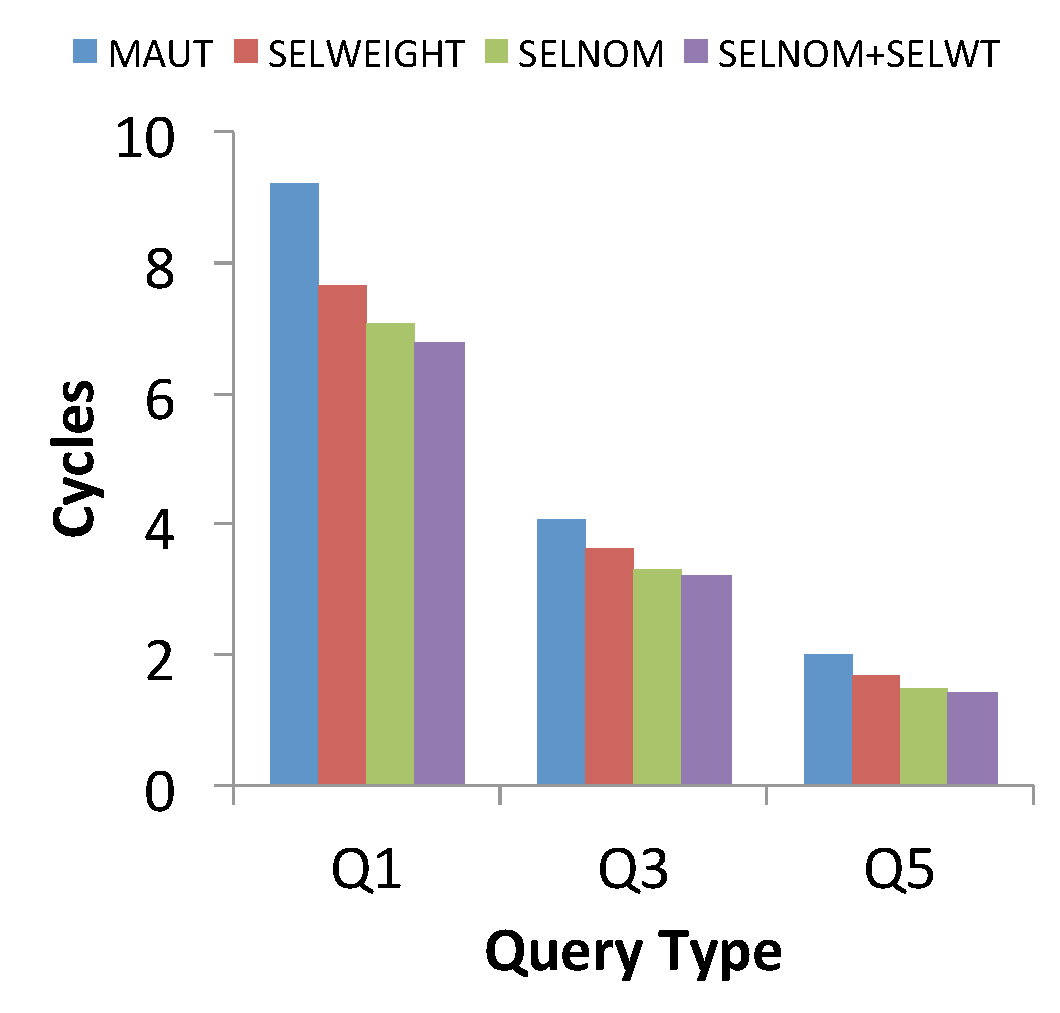
\includegraphics[width=1\linewidth]{figures-bharath/sel_camera_opt}
  \caption[]{Average number of interaction cycles on Camera dataset - optimal user model}
  \label{fig:sel_camera_opt}
\end{minipage}%
\;\;\;\;\;\;
\begin{minipage}{.45\textwidth}
  \centering
  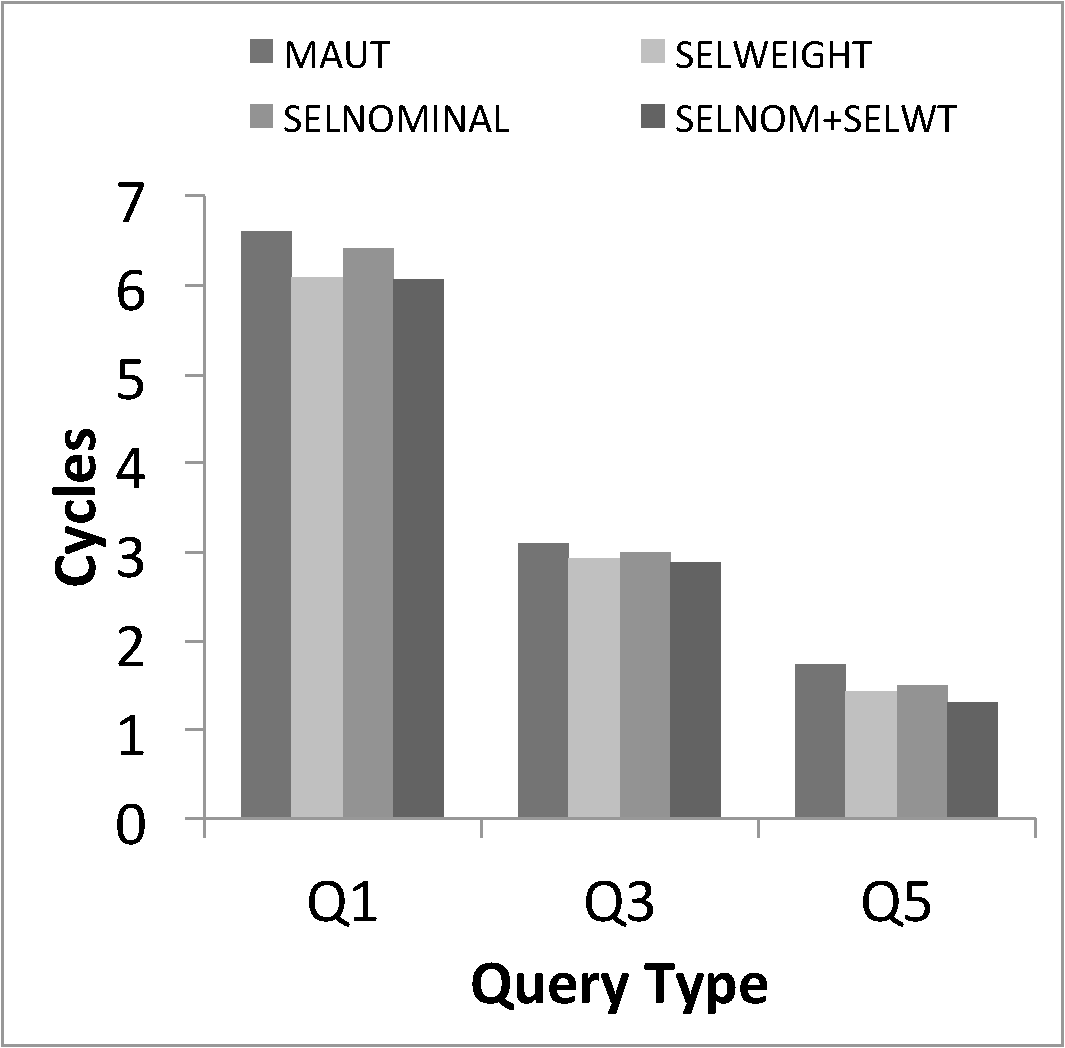
\includegraphics[width=1\linewidth]{figures-bharath/sel_pc_opt}
  \caption[]{Average number of interaction cycles on PC dataset - optimal user model}
  \label{fig:sel_pc_opt}
\end{minipage}
\end{figure}

\begin{figure}[h]
\centering
\begin{minipage}{.45\textwidth}
  \centering
  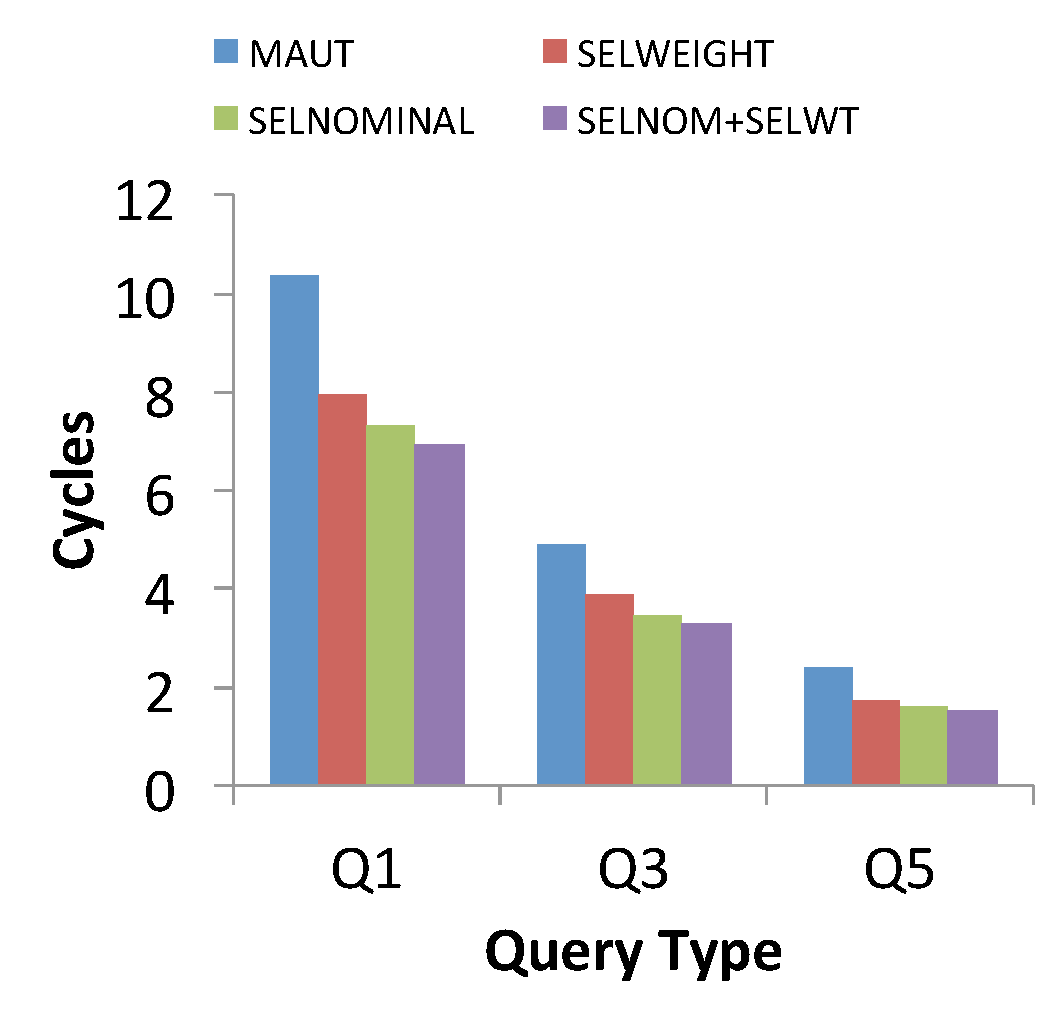
\includegraphics[width=1\linewidth]{figures-bharath/sel_camera_noisy}
  \caption[]{Average number of interaction cycles on Camera dataset - noisy framework}
  \label{fig:sel_camera_noisy}
\end{minipage}%
\;\;\;\;\;\;
\begin{minipage}{.45\textwidth}
  \centering
  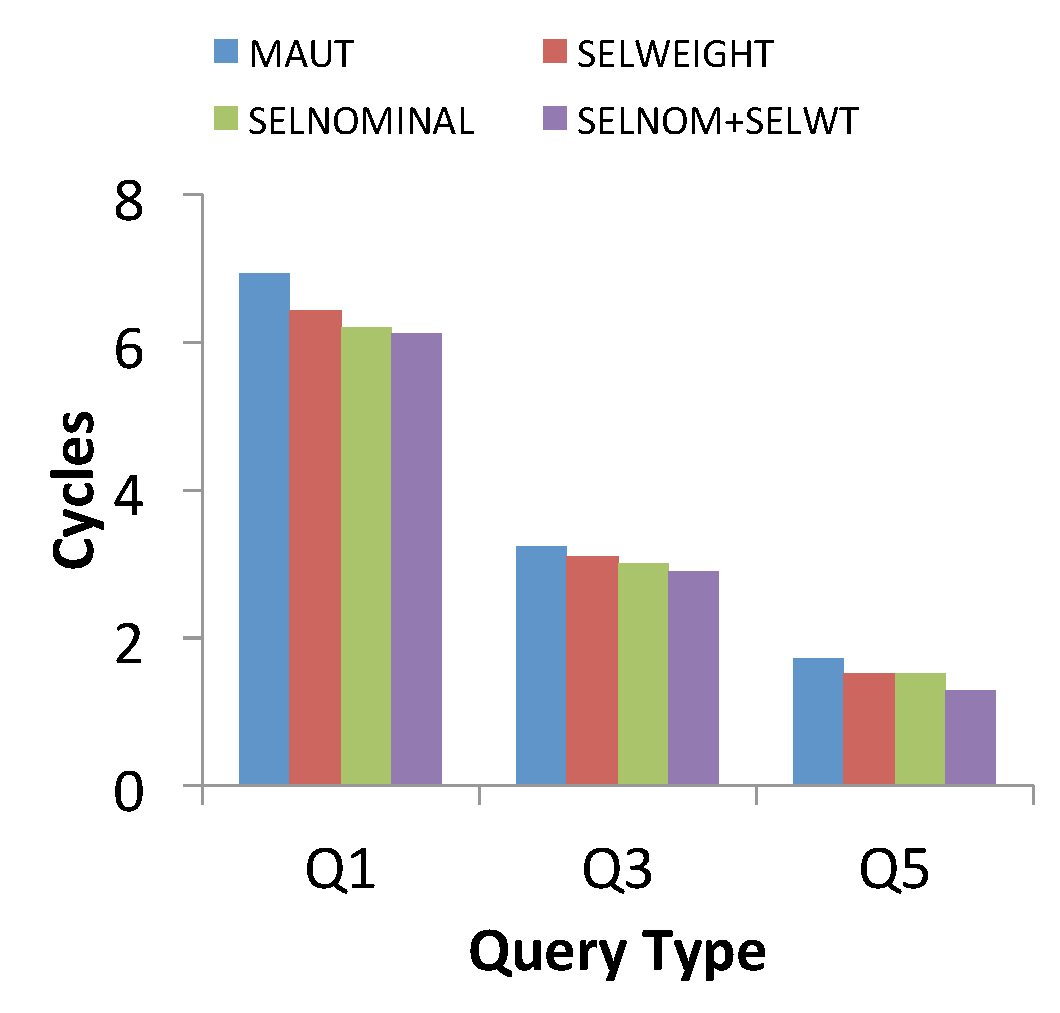
\includegraphics[width=1\linewidth]{figures-bharath/sel_pc_noisy}
  \caption[]{Average number of interaction cycles on PC dataset - noisy framework}
  \label{fig:sel_pc_noisy}
\end{minipage}
\end{figure}
